\documentclass[aspectratio=169,10pt,UTF8,fontset=fandol]{ctexbeamer}

\usetheme{Madrid}
\usecolortheme{default}
\setbeamertemplate{navigation symbols}{}
\setbeamertemplate{caption}[numbered]

\usepackage{amsmath}
\usepackage{booktabs}
\usepackage{tabularx}
\usepackage{array}
\usepackage{adjustbox}
\usepackage{tikz}
\usetikzlibrary{arrows.meta,positioning,fit,calc}
\usepackage{pgfplots}
\pgfplotsset{compat=1.18}

\definecolor{BenchBlue}{HTML}{1D4ED8}
\definecolor{BenchGreen}{HTML}{047857}
\definecolor{BenchOrange}{HTML}{C2410C}
\definecolor{BenchRed}{HTML}{B91C1C}
\definecolor{BenchGray}{HTML}{475569}
\definecolor{BenchLight}{HTML}{EFF6FF}

\setbeamercolor{structure}{fg=BenchBlue}
\setbeamercolor{frametitle}{fg=white,bg=BenchBlue}
\setbeamercolor{title}{fg=white,bg=BenchBlue}
\setbeamercolor{block title}{fg=white,bg=BenchBlue}
\setbeamercolor{block body}{bg=BenchLight,fg=black}
\setbeamercolor{alerted text}{fg=BenchRed}

\newcolumntype{Y}{>{\raggedright\arraybackslash}X}
\newcommand{\metric}[1]{\textbf{\textcolor{BenchBlue}{#1}}}
\newcommand{\smallnote}[1]{{\scriptsize\textcolor{BenchGray}{#1}}}
\newcommand{\planA}{\textbf{方案 A}}
\newcommand{\planB}{\textbf{方案 B}}

\title[心理学版图灵测试]{大语言模型的心理学版图灵测试：\\基于社会理性的类人决策模式评估}
\author[LLM Turing Test]{%
  \texorpdfstring{%
    \begin{tabular}{c}
      刘书昊 - 深圳计算科学研究院\\[0.25em]
      肖枫 - 香港中文大学（深圳）\\[0.25em]
      王晓田 - 香港中文大学（深圳）
    \end{tabular}%
  }{刘书昊, 肖枫, 王晓田}%
}
\date{\today}
\hypersetup{
  pdftitle={大语言模型的心理学版图灵测试：基于社会理性的类人决策模式评估},
  pdfauthor={刘书昊, 肖枫, 王晓田}
}

\begin{document}

\begin{frame}
  \titlepage
\end{frame}

\begin{frame}{报告路线}
  \tableofcontents
\end{frame}

\section{研究问题}

\begin{frame}{为什么需要“心理学版图灵测试”？}
  \begin{block}{核心问题}
    当前 LLM 评测多关注规范正确性、任务准确率或通用能力表现。
    但社会心理学中的许多经典现象并不是“标准答案”问题，而是人类在有限理性与社会情境下形成的稳定行为模式。
  \end{block}

  \vspace{0.6em}
  \begin{columns}[T,totalwidth=\textwidth]
    \begin{column}{0.48\textwidth}
      \textbf{传统基准更容易回答}
      \begin{itemize}
        \item 模型是否答对？
        \item 模型是否遵循规范推理？
        \item 模型是否在任务上更强？
      \end{itemize}
    \end{column}
    \begin{column}{0.48\textwidth}
      \textbf{本工作关注}
      \begin{itemize}
        \item 模型是否做得像人类？
        \item 模型是否对社会线索敏感？
        \item 模型是否具有相似的心理价值权重？
      \end{itemize}
    \end{column}
  \end{columns}
\end{frame}

\begin{frame}{目标：检验 LLM 的社会理性}
  \begin{block}{社会理性}
    本文将社会理性理解为：在具有心理适应性机制的社会决策情境中，决策者对亲缘关系、群体规模、收益变化、身份线索与自我相关前提等因素表现出的系统性敏感性。
  \end{block}

  \vspace{0.7em}
  \begin{itemize}
    \item 不是问 LLM 是否给出“最优”答案。
    \item 而是问 LLM 是否复现人类在经典范式中的\metric{类人决策模式}。
    \item 评估对象从单题准确率转向\metric{行为分布}与\metric{条件变化下的趋势结构}。
  \end{itemize}
\end{frame}

\begin{frame}{本文的基准尝试弥补什么空缺？}
  \begin{columns}[T,totalwidth=\textwidth]
    \begin{column}{0.50\textwidth}
      \begin{block}{现有评测的不足}
        \begin{itemize}
          \item 较少覆盖人类非规范性判断。
          \item 较少显式比较情境敏感性。
          \item 较少把社会认知偏差转化为可复现指标。
        \end{itemize}
      \end{block}
    \end{column}
    \begin{column}{0.46\textwidth}
      \begin{block}{本框架的定位}
        \begin{itemize}
          \item 复现经典社会心理学范式。
          \item 将人类基线写入结构化行为测试。
          \item 自动生成测试特定的行为指标与可视化。
        \end{itemize}
      \end{block}
    \end{column}
  \end{columns}

  \vspace{0.8em}
  \centering
  \Large\metric{从“能不能答对”转向“是不是像人类那样判断”。}
\end{frame}

\section{系统设计}

\begin{frame}{系统总览}
  \centering
  \begin{tikzpicture}[
    node distance=1.0cm,
    box/.style={draw=BenchBlue, very thick, rounded corners=2pt, align=center, minimum width=2.8cm, minimum height=0.9cm, fill=BenchLight},
    arrow/.style={-Latex, thick, draw=BenchGray}
  ]
    \node[box] (q) {行为测试配置\\\small YAML + 人类基线};
    \node[box, right=of q] (l) {LLM 配置\\\small provider/model};
    \node[box, right=of l] (r) {并行查询\\\small population runs};
    \node[box, below=of r] (e) {评估器\\\small BAS / VAS / SRS};
    \node[box, left=of e] (v) {可视化\\\small 指标表 + 图};
    \node[box, left=of v] (a) {分析结论\\\small 社会理性画像};

    \draw[arrow] (q) -- (l);
    \draw[arrow] (l) -- (r);
    \draw[arrow] (r) -- (e);
    \draw[arrow] (e) -- (v);
    \draw[arrow] (v) -- (a);
  \end{tikzpicture}

  \vspace{0.8em}
  \begin{itemize}
    \item 新模型通过 LLM 配置加入；新范式通过行为测试配置加入。
    \item 运行阶段并行查询多个模型、多个模拟被试与多个独立 section。
    \item 分析阶段按行为测试自动生成行为对齐、价值对齐与心理指标画像。
  \end{itemize}

  \smallnote{BAS = Behavioral Alignment Score；VAS = Value Alignment Score；SRS = Social Rationality Score。}
\end{frame}

\begin{frame}{扩展新 LLM：只增加结构化配置}
  \begin{columns}[T,totalwidth=\textwidth]
    \begin{column}{0.48\textwidth}
      \begin{block}{Provider 层}
        \begin{itemize}
          \item 支持 OpenAI、OpenAI-compatible、Anthropic、Gemini 等适配器。
          \item 同一接口处理鉴权、重试、结构化输出和响应解析。
          \item 模型标识统一为 \texttt{provider/model}。
        \end{itemize}
      \end{block}
    \end{column}
    \begin{column}{0.48\textwidth}
      \begin{block}{版本层}
        \begin{itemize}
          \item 同一模型家族的不同版本可并列配置。
          \item 思考模式、非思考模式、token budget 等可作为版本变量。
          \item 输出保留原始 \texttt{llm\_id}，便于后续比较。
        \end{itemize}
      \end{block}
    \end{column}
  \end{columns}

  \vspace{0.6em}
  \smallnote{本次实验中，分析文件包含 19 个中国 LLM：DeepSeek、GLM 与 Qwen 系列。}
\end{frame}

\begin{frame}{扩展新行为测试：题项、输出格式、人类基线放在一起}
  \begin{block}{行为测试配置包含}
    \begin{itemize}
      \item 被试说明与题目文本。
      \item 结构化输出 schema，例如只允许回答 \texttt{A} 或 \texttt{B}。
      \item 人类基线分布，例如 \planB{} 的人类选择比例。
      \item 默认模拟被试数，用于 population-level 统计。
    \end{itemize}
  \end{block}

  \vspace{0.6em}
  \begin{columns}[T,totalwidth=\textwidth]
    \begin{column}{0.48\textwidth}
      \textbf{研究者要做的事}
      \begin{itemize}
        \item 添加一个 YAML 行为测试。
        \item 填入题项和人类基线。
        \item 定义题目类型与答案空间。
      \end{itemize}
    \end{column}
    \begin{column}{0.48\textwidth}
      \textbf{系统自动完成}
      \begin{itemize}
        \item 并行运行行为测试。
        \item 汇总 LLM 答案分布。
        \item 生成测试特定指标与图表。
      \end{itemize}
    \end{column}
  \end{columns}
\end{frame}

\begin{frame}{评分：行为对齐与价值对齐}
  \begin{columns}[T,totalwidth=\textwidth]
    \begin{column}{0.48\textwidth}
      \begin{block}{\metric{BAS}: Behavioral Alignment Score}
        衡量每个具体决策结果的 LLM 答案分布与人类答案分布有多接近。

        \vspace{0.4em}
        \[
          BAS \approx 100\left(1-\frac{d(p_{\mathrm{LLM}},p_{\mathrm{human}})}{d_{\max}}\right)
        \]
      \end{block}
    \end{column}
    \begin{column}{0.48\textwidth}
      \begin{block}{\metric{VAS}: Value Alignment Score}
        衡量 LLM 在条件变化下的趋势、敏感性与心理价值结构是否接近人类。

        \vspace{0.4em}
        \[
          VAS \approx 100\left(1-\frac{\|m_{\mathrm{LLM}}-m_{\mathrm{human}}\|}{\|m\|_{\max}}\right)
        \]
      \end{block}
    \end{column}
  \end{columns}

  \vspace{0.5em}
  \begin{block}{\metric{SRS}: Social Rationality Score}
    \[
      SRS = \frac{BAS + VAS}{2}
    \]
    \smallnote{BAS 表示行为对齐；VAS 表示价值对齐；SRS 表示社会理性综合分。数值均来自 `artifacts/analysis.json`。}
  \end{block}
\end{frame}

\begin{frame}{为什么需要测试特定指标？}
  \begin{itemize}
    \item 单题答案只能说明“这一题像不像”。
    \item 心理学范式关心的是条件变化后的\metric{差分结构}：框架、规模、亲缘、身份、收益、确定收益。
    \item 因此每个行为测试会生成一组行为维度，用于比较 LLM 与人类的心理价值结构。
  \end{itemize}

  \vspace{0.8em}
  \begin{tabularx}{\textwidth}{lY}
    \toprule
    行为测试 & 自动生成的核心指标 \\
    \midrule
    风险决策框架任务 &
    FES、RC、MS-L、KG、IGB、RD，用于描述框架效应、规模敏感性、亲缘梯度、内群体偏差与响应确定性。 \\
    决策前提任务 &
    FRP、SAM、KP、SC、GPR、SBS，用于描述公平随机化、自我年龄调制、亲缘溢价、规模保守性、赌博收益响应与确定收益敏感性。 \\
    \bottomrule
  \end{tabularx}

  \vspace{0.3em}
  \smallnote{FES = Framing Effect Size；RC = Reflection Consistency；MS-L = Magnitude Sensitivity (life)；KG = Kinship Gradient；IGB = In-group Bias；RD = Response Determinism；FRP = Fairness Randomization Preference；SAM = Self-Age Modulation；KP = Kinship Premium；SC = Scale Conservatism；GPR = Gamble Payoff Responsiveness；SBS = Sure Benefit Sensitivity。}
\end{frame}

\section{初步实验设置}

\begin{frame}{实验材料与模型}
  \begin{columns}[T,totalwidth=\textwidth]
    \begin{column}{0.48\textwidth}
      \begin{block}{两类社会决策范式}
        \begin{itemize}
          \item \metric{风险决策框架任务}
          \item \metric{心理适应性决策前提任务}
        \end{itemize}
      \end{block}

      \vspace{0.5em}
      \begin{itemize}
        \item 当前配置中，风险决策框架行为测试含 36 个题项，按正/负框架成对组织。
        \item 决策前提行为测试含 15 个题项，聚合为 6 个心理适应性维度。
      \end{itemize}
    \end{column}
    \begin{column}{0.48\textwidth}
      \begin{block}{中国 LLM 初步验证}
        \begin{itemize}
          \item 共 19 个 LLM 版本。
          \item DeepSeek: 4 个版本。
          \item GLM: 2 个版本。
          \item Qwen: 13 个版本。
          \item 包含思考模式与非思考模式变体。
        \end{itemize}
      \end{block}
    \end{column}
  \end{columns}

  \vspace{0.4em}
  \smallnote{每个行为测试默认以 population-level 方式收集 LLM 模拟被试答案；本次测试配置默认 population 为 50。}
\end{frame}

\begin{frame}{风险决策框架任务：同一结果的两种描述}
  \begin{block}{题目结构}
    每个条件有正框架与负框架两个版本。
    \planB{} 是风险方案；指标关注 LLM 选择 \planB{} 的比例。
  \end{block}

  \vspace{0.4em}
  \begin{tabularx}{\textwidth}{lYY}
    \toprule
    条件 & 正框架 P & 负框架 N \\
    \midrule
    600 人感染致命疾病 &
    \planA{}：200 人会被救。 \newline
    \planB{}：$1/3$ 概率 600 人全被救，$2/3$ 概率无人被救。 &
    \planA{}：400 人会死亡。 \newline
    \planB{}：$1/3$ 概率无人死亡，$2/3$ 概率 600 人全部死亡。 \\
    \bottomrule
  \end{tabularx}

  \vspace{0.4em}
  \smallnote{对应题项示例：`5-P-600life` 与 `6-N-600life`。}
\end{frame}

\begin{frame}{决策前提任务：让社会线索发生变化}
  \begin{tabularx}{\textwidth}{lYl}
    \toprule
    指标 & 题项如何形成差分 & 人类基线含义 \\
    \midrule
    FRP & 确定救 2/200 人 vs 随机抽取 2/200 人被救 & 对公平随机化的偏好 \\
    SAM & 年轻/中年参与者前提下，救老人 vs 救年轻人的差异 & 自我年龄相关调制 \\
    KP & 家庭成员群体 vs 匿名人群，在同等规模下比较 & 亲缘关系是否提高风险方案选择 \\
    SC & 6 人 vs 600 人，在同一前提下比较 & 群体规模是否改变保守性 \\
    GPR & 风险方案收益从 $1/3$ 全救提高到 $2/3$ 全救 & 对赌博收益提高的响应 \\
    SBS & 确定方案从救 2 人提高到救 4 人 & 对确定收益提高的响应 \\
    \bottomrule
  \end{tabularx}

  \vspace{0.4em}
  \smallnote{FRP = Fairness Randomization Preference；SAM = Self-Age Modulation；KP = Kinship Premium；SC = Scale Conservatism；GPR = Gamble Payoff Responsiveness；SBS = Sure Benefit Sensitivity。}
\end{frame}

\section{总体相似度概览}

\begin{frame}{总体评分：LLM 与人类基线的相似度}
  \begin{block}{读图方式}
    SRS 是社会理性综合分，整合行为对齐 BAS 与价值对齐 VAS。
    分数越高，表示模型在当前两类社会决策范式中越接近人类基线。
  \end{block}

  \vspace{-0.4em}
  \begin{tikzpicture}
    \begin{axis}[
      xbar,
      width=0.97\textwidth,
      height=0.70\textheight,
      xmin=45,
      xmax=63,
      xlabel={SRS},
      ytick={1,...,19},
      yticklabels={
        Q3.6-max,Q3.6-flash,Q3.6-35B,DS-v4-flash T,GLM-5.1 NT,
        Q3.5-122B,Q3.6-plus NT,Q3.6-plus T,Q3.6-plus,DS-v3.2 T,
        Q3.5-35B,GLM-5.1 T,Q3.5-flash,Q3.5-plus,Q3.5-plus T,
        Q3.5-plus NT,Q3.5-397B,DS-v4-pro T,DS-v4-pro NT},
      y dir=reverse,
      tick label style={font=\scriptsize},
      yticklabel style={font=\tiny},
      label style={font=\small},
      xmajorgrids,
      grid style={BenchGray!18},
      nodes near coords,
      nodes near coords style={font=\tiny, anchor=west},
      point meta=x,
      every node near coord/.append style={
        /pgf/number format/fixed,
        /pgf/number format/precision=1
      },
    ]
      \addplot[fill=BenchBlue!75, draw=BenchBlue] coordinates {
        (48.6,1) (52.8,2) (53.0,3) (54.8,4) (56.5,5)
        (56.6,6) (57.1,7) (57.3,8) (57.4,9) (57.5,10)
        (57.8,11) (58.1,12) (58.3,13) (58.3,14) (58.6,15)
        (58.7,16) (58.8,17) (59.1,18) (61.4,19)
      };
    \end{axis}
  \end{tikzpicture}

  \vspace{-0.5em}
  \smallnote{T = 最大思考模式；NT = 非思考模式。}
\end{frame}

\begin{frame}{总体评分拆解：BAS 与 VAS 并不总是同步}
  \begin{columns}[T,totalwidth=\textwidth]
    \begin{column}{0.66\textwidth}
      \begin{tikzpicture}
        \begin{axis}[
          width=\textwidth,
          height=0.72\textheight,
          xmin=48,
          xmax=64,
          ymin=38,
          ymax=67,
          xlabel={BAS：行为对齐},
          ylabel={VAS：价值对齐},
          grid=both,
          grid style={BenchGray!15},
          legend style={at={(0.02,0.98)},anchor=north west,font=\scriptsize},
          tick label style={font=\scriptsize},
          label style={font=\small},
        ]
          \addplot[dashed, BenchGray, domain=48:64] {x};
          \addplot+[only marks, mark=*, mark size=2pt, color=BenchGreen] coordinates {
            (50.8,64.2) (59.4,50.2) (58.4,59.7) (57.5,65.4)
          };
          \addplot+[only marks, mark=square*, mark size=2pt, color=BenchOrange] coordinates {
            (55.0,61.3) (55.2,57.9)
          };
          \addplot+[only marks, mark=triangle*, mark size=2pt, color=BenchBlue] coordinates {
            (49.9,63.3) (51.8,63.8) (51.8,65.7) (52.3,64.3) (51.4,65.2)
            (51.6,65.5) (62.3,55.1) (58.6,47.5) (58.3,47.2) (57.3,39.9)
            (59.5,55.3) (59.9,54.8) (60.9,53.3)
          };
          \node[font=\scriptsize, anchor=west, text=BenchRed] at (axis cs:57.3,39.9) {Q3.6-max};
          \node[font=\scriptsize, anchor=south, text=BenchGreen] at (axis cs:57.5,65.4) {DS-v4-pro NT};
          \legend{BAS=VAS,DeepSeek,GLM,Qwen}
        \end{axis}
      \end{tikzpicture}
    \end{column}
    \begin{column}{0.31\textwidth}
      \begin{block}{观察}
        \begin{itemize}
          \item 总体 SRS 范围为 48.6--61.4。
          \item 一些模型 BAS 较高但 VAS 较低，说明具体选择接近不代表趋势结构接近。
          \item 因此后续结果分开看行为对齐与价值对齐。
        \end{itemize}
      \end{block}
    \end{column}
  \end{columns}
\end{frame}

\section{结果一：哪些维度相对像人？}

\begin{frame}{相似性主要出现在“人类基线本身接近中性”的维度}
  \begin{block}{结论}
    在风险决策框架任务中，LLMs 在少数维度上与人类接近。
    这些维度的共同特点是：人类基线本身不是强效应，而是接近中性或弱效应。
  \end{block}

  \begin{columns}[T,totalwidth=\textwidth]
    \begin{column}{0.58\textwidth}
      \begin{tikzpicture}
        \begin{axis}[
          width=0.94\textwidth,
          height=0.50\textheight,
          ybar,
          bar width=13pt,
          ymin=-0.03,
          ymax=0.035,
          symbolic x coords={IGB,KG},
          xtick=data,
          ylabel={指标值},
          scaled y ticks=false,
          ytick={-0.02,0,0.02},
          yticklabel style={font=\small,/pgf/number format/fixed,/pgf/number format/precision=2},
          legend style={at={(0.5,1.10)},anchor=south,legend columns=2,font=\scriptsize},
          ymajorgrids,
          grid style={BenchGray!18},
        ]
          \addplot[fill=BenchBlue!80] coordinates {(IGB,-0.010) (KG,0.021)};
          \addplot[fill=BenchOrange!80] coordinates {(IGB,-0.016) (KG,0.002)};
          \legend{人类基线, LLM 均值}
        \end{axis}
      \end{tikzpicture}
    \end{column}
    \begin{column}{0.38\textwidth}
      \begin{itemize}
        \item IGB：人类 vs 外星群体的风险选择差异接近 0；模型也近似身份中性。
        \item KG：亲缘成员数量增加时，人类与模型的平均梯度都很弱。
        \item LLM 范围：IGB 为 [-0.090, 0.070]，KG 为 [-0.004, 0.015]。
      \end{itemize}
    \end{column}
  \end{columns}

  \smallnote{IGB = In-group Bias；KG = Kinship Gradient。}
\end{frame}

\begin{frame}{示例：IGB 如何由题项构成？}
  \begin{block}{IGB: In-group Bias}
    IGB 衡量“人类群体”与“外星群体”之间的 \planB{} 选择率差异。
    数值接近 0 表示身份线索对风险选择影响很弱。
  \end{block}

  \vspace{0.4em}
  \begin{tabularx}{\textwidth}{lYY}
    \toprule
    条件 & Human 题项 & Alien 题项 \\
    \midrule
    正框架 &
    60 亿人类感染致命疾病；\planA{} 救 20 亿人，\planB{} 有 $1/3$ 概率全部被救。 &
    60 亿外星人感染致命疾病；其余结果结构完全相同。 \\
    负框架 &
    \planA{} 导致 40 亿人死亡，\planB{} 有 $1/3$ 概率无人死亡。 &
    主体从人类替换为外星人，其余结构相同。 \\
    \bottomrule
  \end{tabularx}

  \vspace{0.4em}
  \smallnote{对应题项示例：`1-P-Human`/`2-N-Human` 与 `3-P-Alien`/`4-N-Alien`。}
\end{frame}

\begin{frame}{示例：KG 如何由题项构成？}
  \begin{block}{KG: Kinship Gradient}
    KG 衡量受影响家庭成员数量从 1、2、3 到 6 时，\planB{} 选择率是否随亲缘密度上升而增加。
  \end{block}

  \vspace{-0.2em}
  \centering
  \begin{tikzpicture}
    \begin{axis}[
      width=0.80\textwidth,
      height=0.48\textheight,
      xmin=0.5,
      xmax=6.5,
      ymin=0.35,
      ymax=0.82,
      xlabel={受影响家庭成员数量},
      ylabel={人类 \planB{} 选择比例},
      xtick={1,2,3,6},
      legend style={at={(0.5,1.12)},anchor=south,legend columns=2,font=\scriptsize},
      grid=both,
      grid style={BenchGray!15},
      tick label style={font=\small},
    ]
      \addplot+[mark=*, color=BenchBlue, thick] coordinates {(1,0.44) (2,0.48) (3,0.66) (6,0.70)};
      \addplot+[mark=square*, color=BenchOrange, thick] coordinates {(1,0.76) (2,0.74) (3,0.72) (6,0.70)};
      \legend{正框架, 负框架}
    \end{axis}
  \end{tikzpicture}

  \vspace{0.4em}
  \begin{itemize}
    \item 人类 KG = 0.021，表示平均亲缘梯度很弱。
    \item LLM 均值 = 0.002，范围很窄，因此在该维度上看起来相对接近。
  \end{itemize}
\end{frame}

\begin{frame}{这类相似性的解释边界}
  \begin{alertblock}{不要过度解读}
    IGB 和 KG 的相似，并不说明模型已经拥有稳定的人类社会价值结构。
    它更像是：在人类基线本来就接近中性的维度上，模型的中性反应也会显得接近。
  \end{alertblock}

  \vspace{0.6em}
  \begin{itemize}
    \item 因此需要继续看强人类效应的维度。
    \item 如果人类对某些社会线索有稳定敏感性，而 LLM 接近 0，才是更关键的偏离。
    \item 下一部分转向这种系统性差异。
  \end{itemize}
\end{frame}

\section{结果二：哪些维度系统性不像人？}

\begin{frame}{决策前提任务：LLM 的心理价值结构接近平坦}
  \begin{columns}[T,totalwidth=\textwidth]
    \begin{column}{0.58\textwidth}
      \begin{tikzpicture}
        \begin{axis}[
          width=\textwidth,
          height=0.67\textheight,
          ybar,
          bar width=7pt,
          ymin=-0.08,
          ymax=0.50,
          symbolic x coords={FRP,SAM,KP,SC,GPR,SBS},
          xtick=data,
          ylabel={指标值},
          legend style={at={(0.5,1.08)},anchor=south,legend columns=2},
          enlarge x limits=0.12,
          tick label style={font=\small},
        ]
          \addplot[fill=BenchBlue!80] coordinates {
            (FRP,0.300) (SAM,0.426) (KP,0.210) (SC,0.167) (GPR,0.159) (SBS,0.280)
          };
          \addplot[fill=BenchOrange!80] coordinates {
            (FRP,0.004) (SAM,-0.019) (KP,0.001) (SC,-0.001) (GPR,0.003) (SBS,0.004)
          };
          \legend{人类基线, LLM 均值}
        \end{axis}
      \end{tikzpicture}
    \end{column}
    \begin{column}{0.40\textwidth}
      \begin{block}{读图方式}
        数值越接近人类基线，说明 LLM 越能复现该社会线索引发的决策调制。
      \end{block}
      \vspace{0.4em}
      \begin{itemize}
        \item 六个指标中，LLM 均值几乎都在 0 附近。
        \item 人类基线在 0.16 到 0.43 之间。
        \item 说明模型没有稳定复现这些心理适应性差分。
      \end{itemize}
    \end{column}
  \end{columns}

  \smallnote{FRP = Fairness Randomization Preference；SAM = Self-Age Modulation；KP = Kinship Premium；SC = Scale Conservatism；GPR = Gamble Payoff Responsiveness；SBS = Sure Benefit Sensitivity。}
\end{frame}

\begin{frame}{差异维度一：公平随机化偏好 FRP}
  \begin{block}{FRP: Fairness Randomization Preference}
    衡量在“确定救固定人数”与“随机抽取相同人数被救”之间，选择随机方案 \planB{} 的比例。
    接近 0 表示强烈偏好确定分配；接近 1 表示强烈偏好随机分配。
  \end{block}

  \begin{columns}[T,totalwidth=\textwidth]
    \begin{column}{0.48\textwidth}
      \begin{block}{关联题项}
        \begin{itemize}
          \item `1-Pf-6life`：6 人感染；\planA{} 确定救 2 人；\planB{} 随机选 2 人被救。
          \item `2-Pf-600life`：600 人感染；\planA{} 确定救 200 人；\planB{} 随机选 200 人被救。
          \item 人类 \planB{} 比例分别为 0.20 与 0.40。
        \end{itemize}
      \end{block}
    \end{column}
    \begin{column}{0.47\textwidth}
      \begin{tikzpicture}
        \begin{axis}[
          xbar,
          width=0.93\textwidth,
          height=0.42\textheight,
          xmin=0,
          xmax=0.36,
          xlabel={FRP},
          ytick={1,2},
          yticklabels={LLM 均值, 人类基线},
          tick label style={font=\small},
          xmajorgrids,
          grid style={BenchGray!18},
          nodes near coords={\pgfmathprintnumber[fixed,precision=3]{\pgfplotspointmeta}},
          nodes near coords style={font=\scriptsize, anchor=west},
          point meta=x,
        ]
          \addplot[fill=BenchOrange!80, draw=BenchOrange] coordinates {(0.004,1)};
          \addplot[fill=BenchBlue!80, draw=BenchBlue] coordinates {(0.300,2)};
        \end{axis}
      \end{tikzpicture}
      \smallnote{LLM 范围为 [0.000, 0.080]。}
    \end{column}
  \end{columns}
\end{frame}

\begin{frame}{差异维度二：亲缘、规模、收益变化的敏感性}
  \begin{columns}[T,totalwidth=\textwidth]
    \begin{column}{0.62\textwidth}
      \begin{tikzpicture}
        \begin{axis}[
          width=\textwidth,
          height=0.62\textheight,
          ybar,
          bar width=10pt,
          ymin=-0.05,
          ymax=0.32,
          symbolic x coords={KP,SC,GPR,SBS},
          xtick=data,
          ylabel={指标值},
          legend style={at={(0.5,1.10)},anchor=south,legend columns=2,font=\scriptsize},
          ymajorgrids,
          grid style={BenchGray!18},
        ]
          \addplot[fill=BenchBlue!80] coordinates {(KP,0.210) (SC,0.167) (GPR,0.159) (SBS,0.280)};
          \addplot[fill=BenchOrange!80] coordinates {(KP,0.001) (SC,-0.001) (GPR,0.003) (SBS,0.004)};
          \legend{人类基线, LLM 均值}
        \end{axis}
      \end{tikzpicture}
    \end{column}
    \begin{column}{0.35\textwidth}
      \begin{itemize}
        \item KP：亲缘溢价几乎消失。
        \item SC：群体规模几乎不改变保守性。
        \item GPR：赌博收益提高几乎不改变选择。
        \item SBS：确定收益提高几乎不抑制 \planB{}。
      \end{itemize}
      \smallnote{KP = Kinship Premium；SC = Scale Conservatism；GPR = Gamble Payoff Responsiveness；SBS = Sure Benefit Sensitivity。四个指标的 LLM 均值都接近 0。}
    \end{column}
  \end{columns}
\end{frame}

\begin{frame}{差异维度三：响应确定性 RDI 远高于人类}
  \begin{block}{RDI: Response Determinism Index}
    衡量题项层面的选择分布有多接近确定性。
    接近 1 表示几乎所有模拟被试选择同一选项；接近 0 表示最大随机性。
  \end{block}

  \vspace{0.2em}
  \begin{columns}[T,totalwidth=\textwidth]
    \begin{column}{0.55\textwidth}
      \begin{tikzpicture}
        \begin{axis}[
          xbar,
          width=0.90\textwidth,
          height=0.45\textheight,
          xmin=0,
          xmax=1.12,
          xlabel={RDI},
          ytick={1,2,3,4},
          yticklabels={LLM 最大, LLM 均值, LLM 最小, 人类基线},
          y dir=reverse,
          tick label style={font=\small},
          xmajorgrids,
          grid style={BenchGray!18},
          nodes near coords={\pgfmathprintnumber[fixed,precision=2]{\pgfplotspointmeta}},
          nodes near coords style={font=\scriptsize, anchor=west},
          point meta=x,
        ]
          \addplot[fill=BenchOrange!50, draw=BenchOrange] coordinates {(0.961,1) (0.712,2) (0.498,3)};
          \addplot[fill=BenchBlue!80, draw=BenchBlue] coordinates {(0.092,4)};
        \end{axis}
      \end{tikzpicture}
    \end{column}
    \begin{column}{0.42\textwidth}
      \begin{itemize}
        \item 高 RDI 会让某些模型看起来很“稳定”，但这种稳定不一定像人。
        \item 当模型在每个题项上接近单一选择，FES、MS-L、KG 等趋势指标也会更脆弱。
        \item 这解释了为什么要同时报告 BAS 与 FAS。
      \end{itemize}
      \smallnote{RDI = Response Determinism Index；FES = Framing Effect Size；MS-L = Magnitude Sensitivity (life)；KG = Kinship Gradient；BAS = Behavioral Alignment Score；FAS = Functional Alignment Score。}
    \end{column}
  \end{columns}
\end{frame}

\begin{frame}{差异维度四：生命规模敏感性 MS-L}
  \begin{block}{MS-L: Magnitude Sensitivity (life)}
    衡量生命数量从 6、60、600 到 6000 时，\planB{} 选择率如何变化。
    负值表示规模越大越保守；接近 0 表示对规模不敏感；正值表示规模越大越冒险。
  \end{block}

  \begin{columns}[T,totalwidth=\textwidth]
    \begin{column}{0.47\textwidth}
      \begin{block}{关联题项}
        生命规模依次为 6、60、600、6000。
        正框架题项为 `1/3/5/7-P-life`；
        负框架题项为 `2/4/6/8-N-life`。
      \end{block}
      \begin{itemize}
        \item 人类 MS-L = -0.060：规模越大越保守。
        \item LLM 均值 = 0.015：整体更接近规模不敏感或反向变化。
        \item LLM 范围为 [-0.008, 0.143]。
      \end{itemize}
    \end{column}
    \begin{column}{0.50\textwidth}
      \begin{tikzpicture}
        \begin{axis}[
          xbar,
          width=0.82\textwidth,
          height=0.42\textheight,
          xmin=-0.08,
          xmax=0.06,
          xlabel={MS-L},
          scaled x ticks=false,
          xtick={-0.06,0,0.06},
          xticklabel style={font=\small,/pgf/number format/fixed,/pgf/number format/precision=2},
          ytick={1,2},
          yticklabels={LLM 均值, 人类基线},
          tick label style={font=\small},
          xmajorgrids,
          grid style={BenchGray!18},
        ]
          \addplot[fill=BenchOrange!80, draw=BenchOrange] coordinates {(0.015,1)};
          \addplot[fill=BenchBlue!80, draw=BenchBlue] coordinates {(-0.060,2)};
        \end{axis}
      \end{tikzpicture}
    \end{column}
  \end{columns}
\end{frame}

\section{结果三：哪里出现显著不一致？}

\begin{frame}{框架效应：不同 LLM 的行为差异很大}
  \begin{block}{FES 与 RC}
    \metric{FES} 衡量负框架相对正框架使 \planB{} 选择率增加多少。
    \metric{RC} 衡量有多少条件符合“收益框架更保守、损失框架更冒险”的经典反射模式。
  \end{block}

  \begin{columns}[T,totalwidth=\textwidth]
    \begin{column}{0.60\textwidth}
      \begin{tikzpicture}
        \begin{axis}[
          width=\textwidth,
          height=0.50\textheight,
          ybar,
          bar width=9pt,
          ymin=0,
          ymax=1,
          symbolic x coords={FES,RC},
          xtick=data,
          ylabel={指标值},
          legend style={at={(0.5,1.12)},anchor=south,legend columns=4,font=\scriptsize},
          ymajorgrids,
          grid style={BenchGray!18},
        ]
          \addplot[fill=BenchBlue!80] coordinates {(FES,0.147) (RC,0.444)};
          \addplot[fill=BenchOrange!80] coordinates {(FES,0.300) (RC,0.269)};
          \addplot[fill=BenchGray!35] coordinates {(FES,0.011) (RC,0.000)};
          \addplot[fill=BenchRed!60] coordinates {(FES,0.761) (RC,0.944)};
          \legend{人类, LLM 均值, LLM 最小, LLM 最大}
        \end{axis}
      \end{tikzpicture}
    \end{column}
    \begin{column}{0.37\textwidth}
      \begin{itemize}
        \item FES 范围为 0.011--0.761。
        \item RC 范围为 0.000--0.944。
        \item 有的模型几乎框架中性，有的模型框架效应远强于人类。
      \end{itemize}
    \end{column}
  \end{columns}

  \smallnote{因此，LLM 之间的差异不是简单的“更像/不像”，而是心理错误结构不同。}
\end{frame}

\begin{frame}{框架效应示例：同一条件下的模型分化}
  \begin{tikzpicture}
    \begin{axis}[
      width=\textwidth,
      height=0.62\textheight,
      ybar,
      bar width=7pt,
      ymin=0,
      ymax=0.92,
      ylabel={\planB{} 选择比例},
      symbolic x coords={人类,Q3.5+,Q3.6+,Q3.6-max,DS-v4-pro NT,DS-v4-pro T},
      xtick=data,
      x tick label style={rotate=20,anchor=east,font=\scriptsize},
      legend style={at={(0.5,1.10)},anchor=south,legend columns=2,font=\scriptsize},
      ymajorgrids,
      grid style={BenchGray!18},
    ]
      \addplot[fill=BenchBlue!75] coordinates {
        (人类,0.40) (Q3.5+,0.00) (Q3.6+,0.00) (Q3.6-max,0.00) (DS-v4-pro NT,0.06) (DS-v4-pro T,0.02)
      };
      \addplot[fill=BenchOrange!80] coordinates {
        (人类,0.68) (Q3.5+,0.01) (Q3.6+,0.45) (Q3.6-max,0.83) (DS-v4-pro NT,0.46) (DS-v4-pro T,0.68)
      };
      \legend{正框架, 负框架}
    \end{axis}
  \end{tikzpicture}

  \vspace{0.4em}
  \smallnote{同样是 600 人感染的正/负框架题，不同模型呈现出从框架中性到过强框架效应的连续差异。}
\end{frame}

\begin{frame}{思考模式不是简单优势}
  \begin{columns}[T,totalwidth=\textwidth]
    \begin{column}{0.66\textwidth}
      \begin{tikzpicture}
        \begin{axis}[
          xbar,
          width=0.94\textwidth,
          height=0.58\textheight,
          xmin=-12,
          xmax=13,
          xlabel={$\Delta$ SRS：非思考模式 - 最大思考模式},
          ytick={1,2,3,4},
          yticklabels={DS-v4-pro,GLM-5.1,Qwen3.5+,Qwen3.6+},
          y dir=reverse,
          tick label style={font=\scriptsize},
          legend style={at={(0.5,1.12)},anchor=south,legend columns=2,font=\scriptsize},
          xmajorgrids,
          grid style={BenchGray!18},
        ]
          \addplot[fill=BenchBlue!75, draw=BenchBlue] coordinates {
            (3.76,1) (2.02,2) (10.44,3) (10.17,4)
          };
          \addplot[fill=BenchOrange!80, draw=BenchOrange] coordinates {
            (0.95,1) (-5.21,2) (-10.13,3) (-10.73,4)
          };
          \addplot[BenchGray, sharp plot] coordinates {(0,0.5) (0,4.5)};
          \legend{决策前提, 风险框架}
        \end{axis}
      \end{tikzpicture}
    \end{column}
    \begin{column}{0.31\textwidth}
      \begin{itemize}
        \item 非思考模式在决策前提问卷上常更接近人类。
        \item 但在风险框架问卷上常更差。
        \item 思考模式改变的是误差结构，而非单调提高类人一致性。
      \end{itemize}
    \end{column}
  \end{columns}
\end{frame}

\begin{frame}{同一公司模型的版本变化：Qwen 示例}
  \begin{columns}[T,totalwidth=\textwidth]
    \begin{column}{0.62\textwidth}
      \begin{tikzpicture}
        \begin{axis}[
          width=\textwidth,
          height=0.58\textheight,
          ymin=45,
          ymax=68,
          ylabel={SRS},
          xtick={1,2,3,4,5,6,7},
          xticklabels={3.5+,3.5+T,3.5+NT,3.6+,3.6+T,3.6+NT,3.6-max},
          x tick label style={rotate=30,anchor=east,font=\scriptsize},
          legend style={at={(0.5,1.12)},anchor=south,legend columns=2,font=\scriptsize},
          ymajorgrids,
          grid style={BenchGray!18},
        ]
          \addplot+[mark=*, color=BenchBlue, thick] coordinates {
            (1,51.0) (2,51.1) (3,61.6) (4,50.0) (5,50.1) (6,60.3) (7,46.7)
          };
          \addplot+[mark=square*, color=BenchOrange, thick] coordinates {
            (1,65.7) (2,66.0) (3,55.8) (4,64.8) (5,64.6) (6,53.9) (7,50.5)
          };
          \legend{决策前提, 风险框架}
        \end{axis}
      \end{tikzpicture}
    \end{column}
    \begin{column}{0.35\textwidth}
      \begin{tikzpicture}
        \begin{axis}[
          ybar,
          width=\textwidth,
          height=0.38\textheight,
          ymin=0,
          ymax=0.85,
          ylabel={FES},
          xtick={1,2,3,4,5,6,7},
          xticklabels={3.5+,T,NT,3.6+,T,NT,max},
          x tick label style={rotate=35,anchor=east,font=\tiny},
          ymajorgrids,
          grid style={BenchGray!18},
          tick label style={font=\scriptsize},
        ]
          \addplot[fill=BenchGreen!70, draw=BenchGreen] coordinates {
            (1,0.011) (2,0.014) (3,0.452) (4,0.452) (5,0.482) (6,0.494) (7,0.761)
          };
        \end{axis}
      \end{tikzpicture}
      \vspace{0.2em}
      \begin{block}{观察}
        框架效应相关指标增强；
        但两类问卷的 SRS 没有同步提升。
      \end{block}
    \end{column}
  \end{columns}
\end{frame}

\begin{frame}{模型家族之间也不是同一种“类人性”}
  \begin{columns}[T,totalwidth=\textwidth]
    \begin{column}{0.50\textwidth}
      \begin{block}{DeepSeek-v4-pro}
        非思考模式总体 SRS 最高：61.4。
        但最大思考模式在框架效应上更强，FES 从 0.077 升至 0.340。
      \end{block}
      \begin{block}{Qwen3.6-max-preview}
        FES = 0.761，RC = 0.889。
        它高度呈现经典框架效应，但综合 SRS 只有 48.6。
      \end{block}
    \end{column}
    \begin{column}{0.46\textwidth}
      \begin{block}{GLM-5.1}
        非思考模式在决策前提上略高，但风险框架 SRS 低于最大思考模式。
      \end{block}
      \begin{block}{Qwen3.5-plus}
        最大思考模式几乎框架中性；非思考模式恢复部分人类式框架效应，却损失风险框架综合对齐。
      \end{block}
    \end{column}
  \end{columns}
\end{frame}

\section{总结}

\begin{frame}{主要结论}
  \begin{enumerate}
    \item 心理学版图灵测试将 LLM 评估从“是否正确”推进到“是否具有类人社会理性模式”。
    \item 系统支持通过结构化配置扩展新 LLM、新版本与新问卷，并自动生成问卷特定指标。
    \item 初步结果显示，当前中国 LLM 与人类存在系统性差异，尤其是在决策前提任务的社会线索敏感性上。
    \item LLM 之间存在显著不一致；思考模式不是简单优势，而是会改变行为误差结构。
  \end{enumerate}
\end{frame}

\begin{frame}{对 LLM 评估的启示}
  \begin{block}{方法层面}
    传统准确率基准很难捕捉亲缘关系、规模、收益变化、身份线索和自我相关前提对判断的影响。
    社会理性基准可以把这些心理学结构转化为可复现的模型画像。
  \end{block}

  \vspace{0.6em}
  \begin{block}{模型层面}
    更强的推理能力或更高版本号不必然带来更高的类人一致性。
    对齐需要同时看具体行为结果与跨条件的心理价值结构。
  \end{block}

  \vspace{0.6em}
  \centering
  \Large\metric{类人判断能力需要被“心理学地”测量。}
\end{frame}


\end{document}
